\documentclass[11pt,a4paper]{report}

\usepackage[utf8]{inputenc}
\usepackage[T1]{fontenc}

%%%%%%%%%%% Own packages
\usepackage[a4paper, margin=1in]{geometry}

% Boxing
\usepackage[most]{tcolorbox}
\tcbset{enhanced}
%\usepackage{capt-of}	% captions in boxes

% Header/footer
\usepackage{fancyhdr}
\pagestyle{fancy}
\renewcommand{\headrulewidth}{0pt}

% Listsings and items
\usepackage{enumerate}

% Maths
\usepackage{physics}
\usepackage{cancel}

\usepackage{caption}
\captionsetup{margin=10pt,font=small,labelfont=bf}
%\renewcommand{\thesubfigure}{(\alph{subfigure})} % Style: 1(a), 1(b)
%%%%%%%%%%%

%\pagestyle{empty}

\usepackage{graphicx}% Include figure files
%\usepackage{epstopdf}
%\usepackage{pdfsync}
\usepackage{amstext,amsbsy}
\usepackage{times} 

%% Numbered problems
\newcounter{excount}[chapter]
\newenvironment{exercise}[1][]{\addtocounter{excount}{1} \noindent {\bf Problem
    \arabic{excount} \ \ #1}\hspace{2mm}}{\vspace{4mm}}

%% Solution environment
\newenvironment{solution}
    {\begin{tcolorbox}[title=Solution,halign lower=right,breakable]
    }
    {
    \tcblower Jakob Borg
    \end{tcolorbox}
	\vspace{5mm}
    }

%% Figure command
\newcommand{\fig}[2][]
{
\begin{center}
\includegraphics[width=0.49\linewidth]{#2}
\captionof{figure}{#1}
\label{fig:fig\arabic{figure}}
\end{center}
}

%% Quichalf
\newcommand{\half}
{
\frac{1}{2}
}

\title{FYS3120 Classical Mechanics and Electrodynamics\\ 
\vspace{15mm}Problem set 1}
\author{Jakob Borg}

%%%%%%%
\begin{document}
%%%%%%%

\maketitle

%\lhead{Jakob Borg}
\lhead{Problem set 1 FYS3120}
\rhead{Jakobbor}
%%%%%%%%

\begin{exercise}
Figure~\ref{fig:fig1} shows four different mechanical systems, in {\bf a)} a pendulum attached to a block which in turn is attached to a spring, {\bf b)} a pendulum which is attached to a vertical ring which rotates with a fixed frequency $\omega$, {\bf c)} a straight rod which can tilt without sliding on the top of cylinder, while the cylinder can roll on a horizontal plane (no slipping), and {\bf d)} a spinning top which moves on a horizontal floor.

In all cases specify the number of degrees of freedom and choose an appropriate set of generalized coordinates.

\begin{solution}
\begin{center}
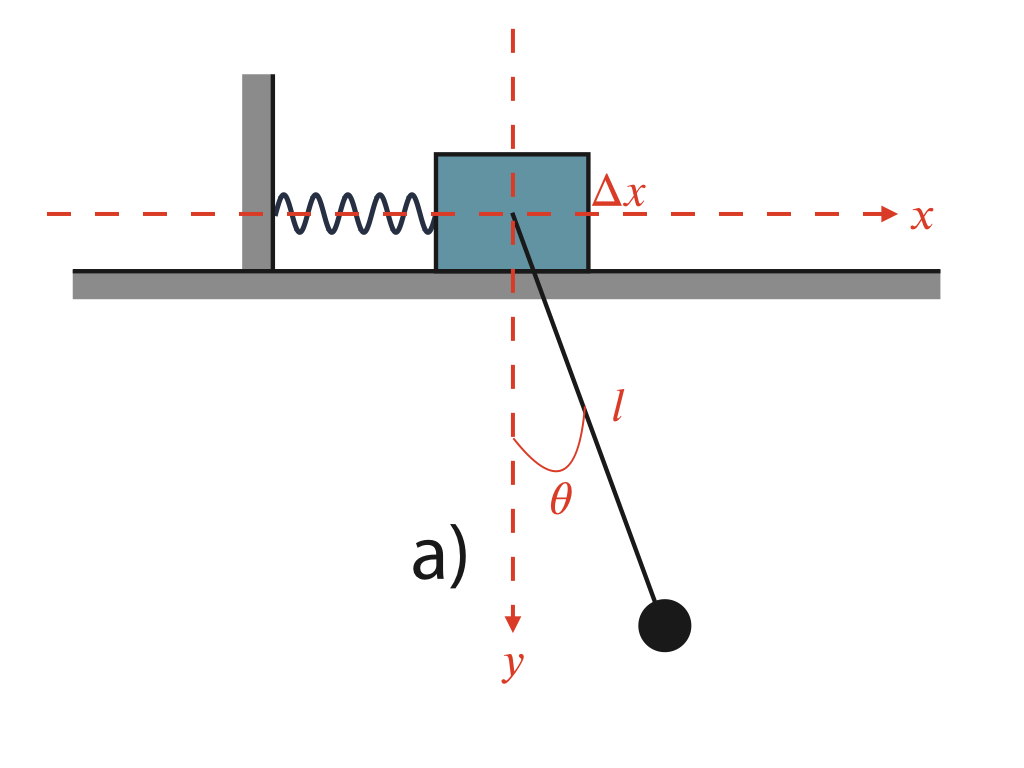
\includegraphics[width=0.49\linewidth]{./vectorfigurer/fig_001.png}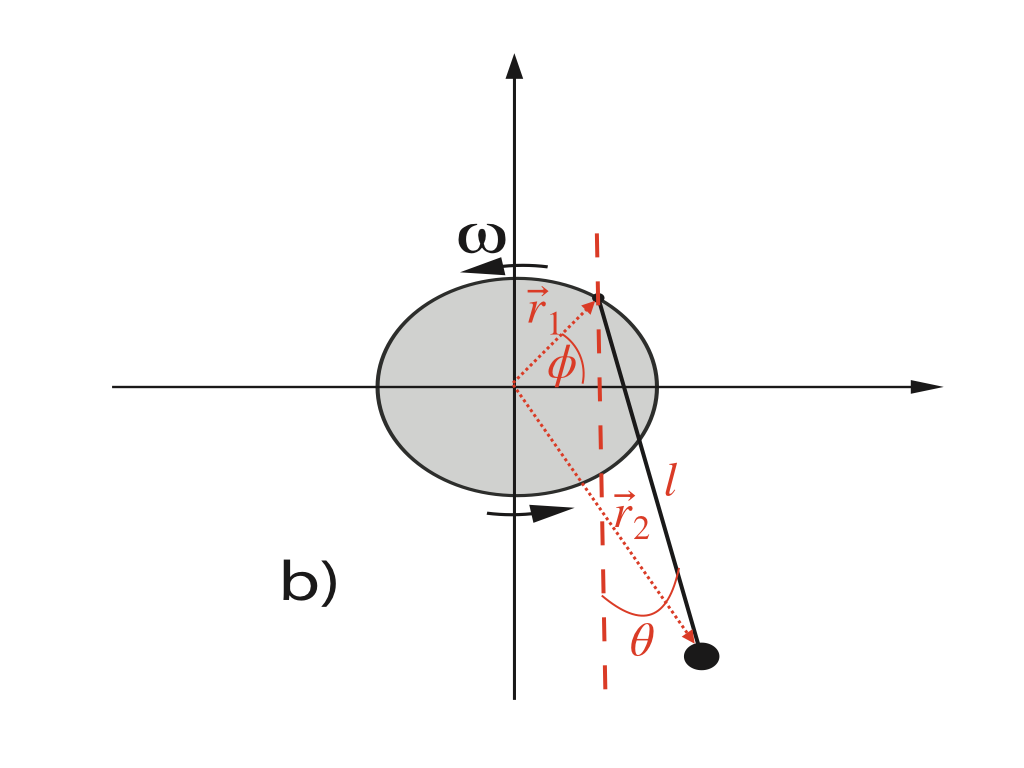
\includegraphics[width=0.49\linewidth]{./vectorfigurer/fig_002.png}	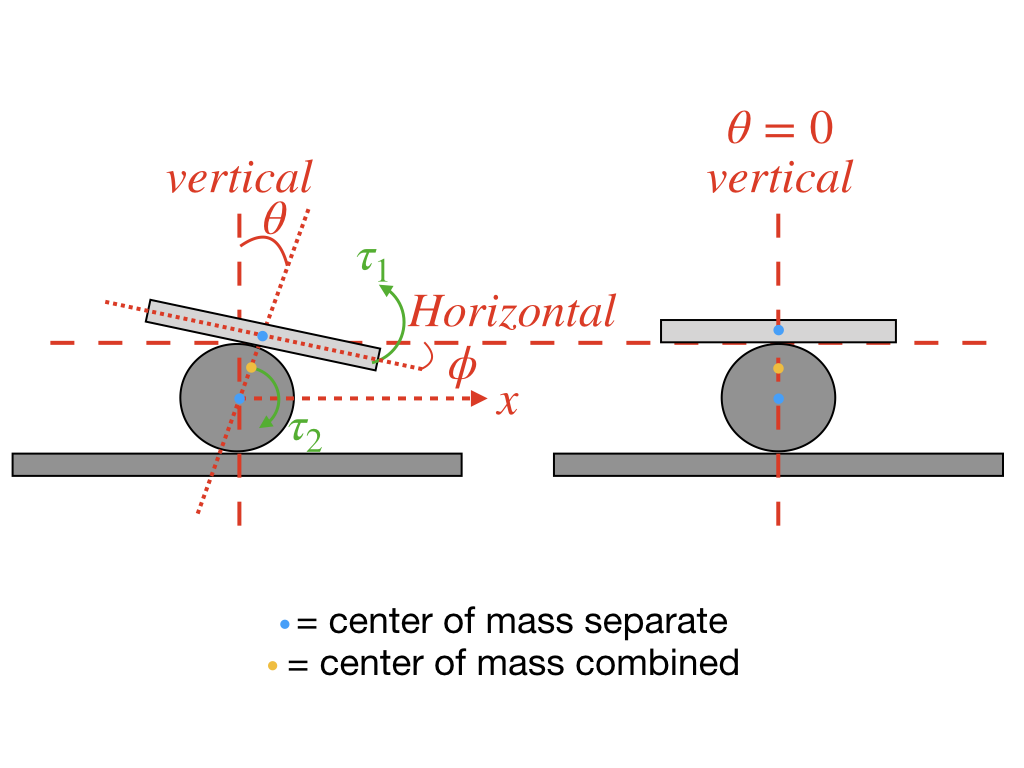
\includegraphics[width=0.49\linewidth]{./vectorfigurer/fig_003.png}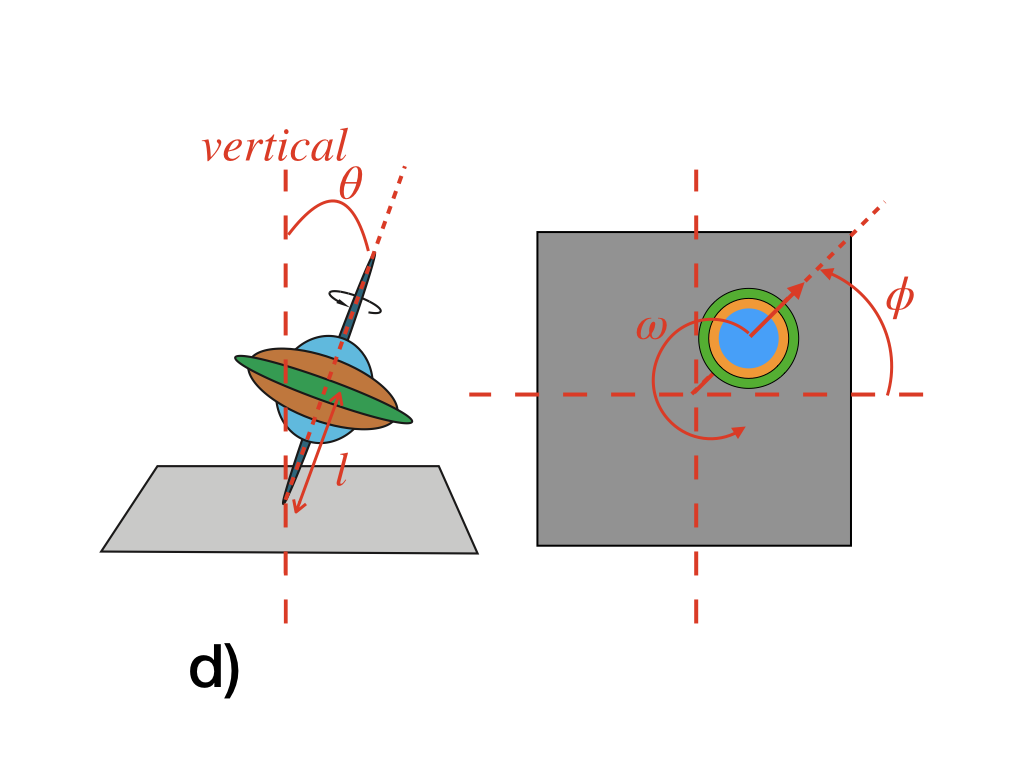
\includegraphics[width=0.49\linewidth]{./vectorfigurer/fig_004.png}
\captionof{figure}{Four different mechanical systems}\label{fig:fig1}
\end{center}
In this problem I'm a bit unsure in what detail we are asked to describe the systems, and what classifies as <<specify>> the number of degrees of freedom. As this is the first problem set I have tried some different approaches to listing and discussing the different systems.
\begin{enumerate}[a)]
	\item Here I assume the box to be fixed to the surface and that there is no max extension of the spring. I then need one coordinate to describe the displacement of the box from the equilibrium position, $\Delta x$, and two coordinates $x$ and $y$ for the pendulum. With one constrain; $\abs{x-y} -l = 0$, that results in two generalized coordinates, and I choose the set $q = \qty{\Delta x, \theta}$.
	\item Let $r$ be the radius of the disc. With $\omega$ fixed I find the number of degrees of freedom to be:
	\begin{align*}
	+2& \qq{coords for the attachment point} &\va{r}_1 = x_1\vu{i}+y_1\vu{j}
	\\
	+2& \qq{coords for the pendulum} &\va{r}_2 = x_2\vu{i}+y_2\vu{j}
	\\
	-2& \qq{from constraints} &\abs{\va{r}_1} - r = 0\qc \abs{\va{r}_2} - l = 0
	\\
	\hline
	2& \qq{generalized coords} & q = \qty{\phi,\theta}
	\end{align*}
	\item Here I assume the system to be balanced, because if the system at one point falls apart by the rod touching the ground this would introduce a non-holonomic constraint. For the system to be balanced requires that there is a point in time where the rod lie perfectly horizontal on top of the cylinder, with the rod's and cylinder's center-of-mass along the same vertical line. The motion of the system then oscillates between two extreme points with the $\theta = 0$ state in the middle. When the cylinder rolls to one side, with no sliding between the plane or the rod, the contact point between the cylinder and the rod will move along the top of the cylinder the exact same distance as the cylinder moves along the surface, call it $s$. As there are no slipping, the contact point will always be at the center-of-mass of the rod, according to my assumptions.

To describe the horizontal movement $\Delta x$ of the disc I will use the angular displacement $\theta$ from the vertical, with zero at the equilibrium point where the rod is perfectly horizontal, together with the radius of the cylinder, $\Delta x =s =  \theta r$. When the cylinder moves, the center of mass of the rod moves with it, so that the combined center of mass is off the vertical axis. This will introduce a torque on the system $\tau_2$ due to gravity. For my balance criteria this has to be counteracted by the torque from the rotational motion of the rod, $\tau_1$ for the system to balance out and move back to the equilibrium position. Here I am a bit uncertain, but I think this criteria is enough to find a dependence between the angle $\theta$ and $\phi$ (I have drawn this angle too in the figure) using the inertia of the rod and the cylinder. 

Resulting set $q = \qty{\theta}$.
	
	
	To be able to describe systems that start out in an unbalanced state I would also need the angle $\phi$, describing a possible tilt of the rod off the horizontal line at the $\theta = 0$ state.
	\item I will assume we neglect the motion of the contact point with the floor, as to describe this motion we have to include friction, which is non-conservative, and introduce energy loss to the system. This would inevitably cause the spinning top to slow down and be a much more complicated system. Therefor I will describe the spinning top relative to the contact point with the floor, and to do that I need three coordinates to position the center-of-mass. With one constrain; the length from the contact point to the center-of-mass is $l$, this gives $d=3-1=2$ degrees of freedom. With a rotating system i choose the set $q = \qty{\phi,\theta}$ as generalized coordinates.
\end{enumerate}
\end{solution}
\end{exercise}
%%%%%%%%



%%%%%%%%
\begin{exercise}
An Atwood machine consists of three parts, with masses $m_1=4m$, $m_2=2m$ and $m_3=m$, that move vertically, and two rotating pulleys, which we treat as massless.  The fixed lengths of the ropes, which we also consider as massless, are $l_1$ and $l_2$. We show the set-up in Fig.~\ref{fig:fig2}.

Explain why the number of degrees of freedom of the system is two and choose a corresponding set of generalized coordinates. Find the potential and kinetic energies of the system expressed as functions of the generalized coordinates and their time derivatives. Write down the Lagrangian of the system.

\begin{solution}
\fig[An Atwood machine with three masses. I choose the zero point of y at the height where the lower pulley and $m_1$ are leveled, this is also where $\alpha = 0$. OBS: Error in the original figure, both ropes are indicated as $l_2$, I treat the lower of the two as $l_2$.]{./vectorfigurer/fig_005.png}
\subsubsection*{D.o.f.}
Let $r$ be the radius of the two pulleys. I will assume equal radii, but with the choice of coordinates I'm going to make it's easily extended to two different radii. I will also ignore the position of the upper pulley as it's fixed.
\begin{align*}
	+4 & \cdot 2 \qq{coords for each mass and lower pulley} &\va{r}_i = x_i\vu{i} + y_i\vu{j}
	\\
	-4 & \qq{fixed $x$ position for each <<particle>>}
	\\
	-2 & \qq{fixed lengths of each rope}
	\\
	\hline
	2 & \qq{generalized coords} & q = \qty{\alpha,\beta}
\end{align*}
I choose to use the angular rotation of each pulley as the generalized coordinates. I've oriented the y-axis downwards, with positive orientation of the angles against the clock. It's easily converted from vertical position using $s = r\theta$, and can easily be extended to problems where the two pulleys have different radii as mentioned. Using these coordinates is also advantageous if we want to give the pulleys mass and inertia.
\subsection*{Energy}
I need to express the position and velocity of each mass, I will only look at vertical displacement.
\begin{equation*}
	\va{r}_1 = \alpha r \vu{j} \qc v_1^2 = \abs*{\dot{\va{r}}_1}^2 = \qty (\dot{\alpha}r)^2
\end{equation*}
The masses $m_2$ and $m_3$'s positions are affected by the movement of the lower pulley, that is the opposite of the movement of $m_1$, and adjusted by the length of the lower rope.
\begin{align*}
	\va{r}_2 &= \qty(\frac{l_2}{2}+r\qty(\beta-\alpha))\vu{j} \qc v_2^2 = r^2\qty(\dot{\beta} - \dot{\alpha})^2
	\\
	\va{r}_3 &= \qty(\frac{l_2}{2}-r\qty(\beta+\alpha))\vu{j} \qc v_3^2 = r^2\qty(\dot{\beta} + \dot{\alpha})^2	
\end{align*} 
\subsubsection*{Kinetic}
\begin{align*}
	K &= \frac{1}{2}m_1v_1^2 + \half m_2 v_2^2 + \half m_3v_3^2
	\\
	&= mr^2\qty(2\dot{\alpha}^2 + \qty(\dot{\beta}-\dot{\alpha})^2 + \half \qty(\dot{\beta} + \dot{\alpha})^2)
	\\
	&= mr^2 \qty( \frac{7}{2}\dot{\alpha}^2 + \frac{3}{2}\dot{\beta}^2 - \dot{\beta}\dot{\alpha})
\end{align*}
\subsubsection*{Potential}
With the zero point at $y=0$. This will introduce a constant in the potential energy from the two lower pulleys hanging $\frac{l_2}{2}$ below the zero. I will just neglect these terms as it is an uninteresting constant, and modifying the zero point to account for this removes the contribution.
\begin{align*}
	V &= -g \qty ( m_1y_1 + m_2y_2 + m_3y_3)
	\\
	&= -mg \qty(4r\alpha + 2\qty(\cancel{\frac{l_2}{2}} + r\qty(\beta - \alpha)) + \cancel{\frac{l_2}{2}} -r\qty(\beta+ \alpha))
	\\
	&= mgr \qty(\beta+\alpha)
\end{align*}
\subsubsection*{Lagrangian}
One way to express the Lagrangian is then
\begin{align*}
	L &= mr^2 \qty(\frac{7}{2}\dot{\alpha}^2+\frac{3}{2}\dot{\beta}^2 -\dot{\beta}\dot{\alpha}) + mgr\qty(\beta + \alpha)
\end{align*}
\end{solution}
\end{exercise}
%%%%%%%%

%%%%%%%%
\begin{exercise}
Three identicals rods of mass $m$ and length $l$ are connected by frictionless joints and suspended,  with the distance between the points of suspension being equal to the length of the rods, as shown in Fig.~\ref{fig:fig3}. The rods move in the plane. Explain why the system has only one degree of freedom, and choose the angle $\theta$ as generalized coordinate.

Show that the Lagrangian, defined as the difference between the kinetic and potential energy, $L=K-V$, gets the following form as a function of $\theta$ and $\dot\theta$,
\begin{equation}
L(\theta,\dot\theta)={5\over 6}m l^2\dot\theta^2+2mgl\cos\theta.
\end{equation}
We remind you that the expression for the moment of of inertia of a rod about its endpoint is $I={1\over 3}m l^2$.
\end{exercise}
%%%%%%%%

\begin{solution}
\fig{./vectorfigurer/fig_006.png}
One may describe the system of three rods as three pendulums, connected to each other at the end points so that they move fixed together. As we know, a pendulum may be described by a single coordinate, for example the angle of the vertical axis $\theta$. Using this we may describe the motion of one of the three rods with $\theta$, and as the other two rods positions are fixed according to the first pendulum, we are in fact describing the hole system.

\subsection*{Energy}
The two vertical rods rotate around their endpoint resulting in rotational kinetic energy. The third horizontal rod may be viewed as a series of small pendulums hanging in mass less rods. For simplicity, I will think of it as a single pendulum from a mass less rod located at the rod's center of mass, contributing kinetic energy as a normal pendulum.
\subsubsection*{Kinetic}
\begin{align*}
	K &= 2 \cdot \frac{1}{2}I \omega^2 + \frac{1}{2}mv^2 
	= \frac{1}{3}ml^2 \dot{\theta}^2 + \frac{1}{2}m\qty(l\omega)^2
	\\
	&= \frac{5}{6}m\qty(l\dot{\theta}^2)
\end{align*}
\subsubsection*{Potential}
Let the zero point be at $y=0$, that is when $\theta = 0$. The two vertical rods will then contribute to the potential energy even when the systems stands still at equilibrium as their center-of-mass is higher than the zero point. But this will only introduce some constant value that may be neglected at the end.
\begin{align*}
	V &=2mg\qty(\frac{l}{2}+\frac{l}{2}\cos \theta) + mgl\cos \theta
	\\
	&= 2mgl\cos \theta + \cancel{mgl}
\end{align*}
\subsubsection*{Lagrangian}
This results in a Lagrangian on the form
\begin{equation*}
	L = K - V = \frac{5}{6}ml^2\dot{\theta}^2 + 2mgl\cos \theta
\end{equation*}
as wanted.

\end{solution}


%%%%%%%%
\begin{exercise}
A particle with mass $m$ moves in three-dimensional space under the influence of a constraint. The constraint is expressed by the equation
\begin{equation}
e^{-(x^2+y^2)}+z=0,
\end{equation}
for the Cartesian coordinates $(x,y,z)$ of the particle.
\begin{itemize}
\item[\bf a)]Explain why the number of degrees of freedom of the particle is two. Use $x$ and $y$ as generalized coordinates and find the expression for the position vector $\vec r$ of the particle in terms of $x$ and $y$. 
\item[\bf b)]A virtual displacement is a change in the position of the particle $\vec r \to \vec r + \delta \vec r$ which is caused by an inifinitesimal change in the generalized coordinates, $x \to x + \delta x$ and $y\to y+\delta y$. Find $\delta \vec r$ expressed in terms of $\delta x$ and $\delta y$.
\item[\bf c)]The constraint can be interpreted as a restriction for the particle to move on a two-dimensional surface in three-dimensional space. Any virtual displacement $\delta \vec r$ is a tangent vector to the surface while the constraint force $\vec f$ which acts on the particle is perpendicular to the surface. Use this to determine $\vec f $ (up to a normalization factor) as a function of $x$ and $y$.
\item[\bf d)]Make a drawing of a section through the surface for $y=0$. Indicate in the drawing the direction of the two vectors $\vec f$ and $\delta \vec r$ for a chosen point on the surface.
\end{itemize}

\begin{solution}

\begin{enumerate}[a)]
	\item With $N=1$ particle and $M=1$ constraint this results in two d.o.f.
	\begin{align*}
	d &= 3N -M = 2
	\end{align*}
	This can be thought of as the particle being free to move in two dimensions, $x$ and $y$, while the $z$ component is controlled by the constraint resulting in a 2D configuration space. The position may be expressed as
	\begin{align*}
	\va{r} &= x\vu{i} + y\vu{j} + z \vu{k} = x\vu{i} + y\vu{j} - e^{-\qty(x^2+y^2)} \vu{k}
	\end{align*}
	\item The virtual displacement is defined as
	\begin{align*}
	\var{\va{r}} &= \sum_{j=1}^d \pdv{\va{r}}{q_j}\var{q}_j \qq{where} q = \qty{x,y} \qc d=2
	\\
	&= \pdv{\va{r}}{x} \var{x} + \pdv{\va{r}}{y}\var{y}
	\\
	&= \qty(\vu{i} +2xe^{-\qty(x^2+y^2)}\vu{k})\var{x} + \qty(\vu{j} + 2ye^{-\qty(x^2+y^2)}\vu{k})\var{y}
	\end{align*}
	\item I can find an expression for the constraint force, up a normalization factor, by utilizing that it does no virtual work.
	\begin{align*}
	&\va{f} \cdot \delta\va{r} = 0
	\\
	&\qty( f_x\vu{i} + f_y\vu{j} + f_z\vu{k} ) \cdot \qty[ \qty( \vu{i} +2xe^{-\qty(x^2+y^2)}\vu{k} ) \var{x} + \qty( \vu{j} + 2ye^{-\qty(x^2+y^2)}\vu{k} )\var{y} ] = 0
	\\
	&\qq*{as} \delta x,\, \delta y \qq{are independent these two equations can be solved independently}
	\\
	&f_y + f_z2ye^{-\qty(x^2+y^2)}  = 0 \Rightarrow f_z = - \frac{f_y}{2ye^{-\qty(x^2+y^2)}}
	\\
	&f_x + f_z2xe^{-\qty(x^2+y^2)} = 0 \Rightarrow f_x - \frac{f_y}{2ye^{-\qty(x^2+y^2)}}2xe^{-\qty(x^2+y^2)} = f_x - f_y \frac{x}{y} = 0
	\\
	&\va{f} = f_y \qty(\frac{x}{y} \vu{i} + \vu{j} - \frac{1}{2ye^{-\qty(x^2+y^2)}}\vu{k})
	\end{align*}
	up to the normalization factor $f_y$.
	\item Sketch in Fig. \ref{fig:fig4}.
	\fig[Sketch of the surface for $y=0$. The $\delta \va{r}$ is tangent to the surface, and $\va{f}$ is normal to the surface.]{./vectorfigurer/fig_007.png}
\end{enumerate}

\end{solution}
\end{exercise}
%%%%%%%%

%%%%%%%%%
%\begin{exercise}
%A flexibel chain can move without friction on a smooth surface, as shown in Fig.~\ref{fig:chain}. It has constant mass density along the chain. The vertical heigths of the end points are $z_A$ and $z_B$. Use the principle of virtual work to find how $z_A$ and $z_B$ are related when the chain is in static equilibrium.
%
%\begin{figure}[h!]
%\begin{center}
%\includegraphics[width=7cm]{VirtualWork.eps}
%\end{center}
%\caption{Flexible chain.}
%\label{fig:chain}
%\end{figure}
%
%\end{exercise}
%%%%%%%%


%%%%%%
\end{document}
%%%%%%%%
